\section{Antecedentes}
\label{section:antecedentes}
\noindent\textbf{Vida artificial}

Craig W. Reynolds, publica “Steering Behaviors For Autonomous Characters” en este trabajo se explica la forma de crear un modelo computacional para el movimiento 
coordinado de grupos de caracteres autónomos (llamados boids).
 
Estas entidades son capaces de moverse por su mundo de una manera improvisada y realista. Para ello el modelo tiene que respetar ciertas reglas que aseguren las condiciones reales 
del movimiento de caracteres coordinados. Siendo las dos reglas más importantes las siguientes:
No puede existir una inteligencia superior al resto.
Cada entidad se mueve de modo independiente según las reglas del modelo y su ponderación respectiva.
 
Gracias a estas reglas, y modificando los valores ponderables de los comportamientos la simulación se asemejara mucho a la conducta real de diferentes especies, desde bancos de 
peces a bandadas de aves. Existiendo siempre una cohesión para que se desplacen en manada, una alineación para que se dirijan en la misma dirección y una separación para evitar que
choquen los unos con los otros.
 
Además, aunando diferentes comportamientos se pueden crear otros mas complejos que pueden dar lugar a situaciones donde las entidades sean capaces de evitar obstáculos del mundo o 
seguir un camino prefijado como una manada.
 
Algunas de las características más importantes del modelo son: la falta de predictibilidad en un lapso de tiempo considerable y la formación de comportamientos emergentes, es decir, 
que no están planeados y que pueden sorprender al propio creador.\\

\noindent\textbf{Audio}

Ha habido varios intentos de crear una potente API de audio para la Web y así,  hacer frente a algunas de las limitaciones que se han descrito anteriormente.  Un ejemplo notable es el Audio Data API,  que fue diseñado y prototipo en Mozilla Firefox.  El enfoque de Mozilla comenzó con un elemento $<$audio$>$, y amplió su API de JavaScript con características adicionales. Esta API tiene un gráfico de audio limitado, y no se ha adoptado más allá de su primera aplicación. Se ha quedado en desuso en la actualidad en Firefox a favor de la Web Audio API [Figura \ref{fig:../images/versiones_navegadores.png}].

\begin{figure}
 \centering
 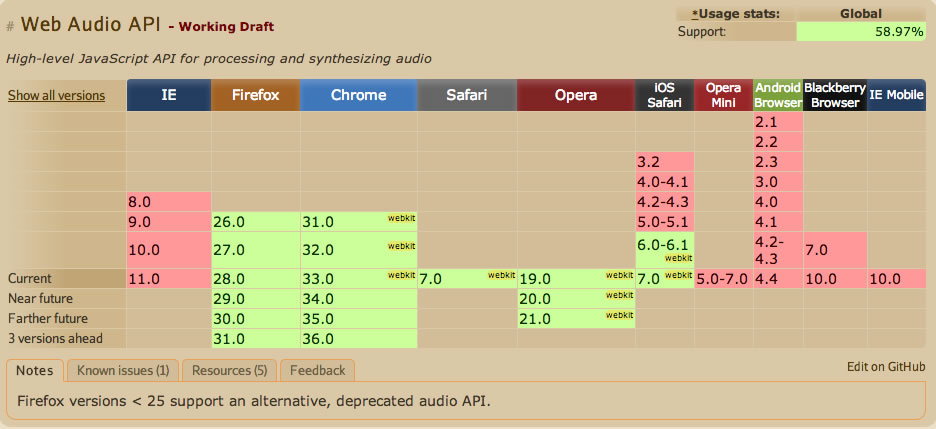
\includegraphics[width=\textwidth]{../images/versiones_navegadores.png}
 \caption{Comparativa de las versiones de los navegadores que soportan a Web Audio API}
 % versiones_navegadores.png: 936x429 pixel, 72dpi, 33.02x15.13 cm, bb=0 0 936 429
 \label{fig:../images/versiones_navegadores.png}
\end{figure}


En contraste con Audio Data API, la Web Audio API es un nuevo modelo de la marca, totalmente independiente de la etiqueta $<$audio$>$,  aunque hay puntos de integración con otras API de Web. Se trata de una API de alto nivel JavaScript para la transformación y síntesis de audio en aplicaciones web. El objetivo de esta API,  es incluir capacidades que se encuentran en los motores de juego modernos,  y algunas de las tareas de mezcla, tratamiento y filtrado que se encuentran en aplicaciones de producción de audio de escritorio modernos. El resultado es una API versátil que se puede utilizar en una variedad de tareas relacionadas con el audio y visualizaciones de síntesis de música muy avanzadas.